\IfFileExists{stacks-project.cls}{%
\documentclass{stacks-project}
}{%
\documentclass{amsart}
}

% For dealing with references we use the comment environment
\usepackage{verbatim}
\newenvironment{reference}{\comment}{\endcomment}
%\newenvironment{reference}{}{}
\newenvironment{slogan}{\comment}{\endcomment}
\newenvironment{history}{\comment}{\endcomment}

% For commutative diagrams we use Xy-pic
\usepackage[all]{xy}

% We use 2cell for 2-commutative diagrams.
\xyoption{2cell}
\UseAllTwocells

% We use multicol for the list of chapters between chapters
\usepackage{multicol}

% This is generally recommended for better output
\usepackage{lmodern}
\usepackage[T1]{fontenc}

% For cross-file-references
\usepackage{xr-hyper}

% Package for hypertext links:
\usepackage{hyperref}

% For any local file, say "hello.tex" you want to link to please
% use \externaldocument[hello-]{hello}
\externaldocument[introduction-]{introduction}
\externaldocument[conventions-]{conventions}
\externaldocument[sets-]{sets}
\externaldocument[categories-]{categories}
\externaldocument[topology-]{topology}
\externaldocument[sheaves-]{sheaves}
\externaldocument[sites-]{sites}
\externaldocument[stacks-]{stacks}
\externaldocument[fields-]{fields}
\externaldocument[algebra-]{algebra}
\externaldocument[brauer-]{brauer}
\externaldocument[homology-]{homology}
\externaldocument[derived-]{derived}
\externaldocument[simplicial-]{simplicial}
\externaldocument[more-algebra-]{more-algebra}
\externaldocument[smoothing-]{smoothing}
\externaldocument[modules-]{modules}
\externaldocument[sites-modules-]{sites-modules}
\externaldocument[injectives-]{injectives}
\externaldocument[cohomology-]{cohomology}
\externaldocument[sites-cohomology-]{sites-cohomology}
\externaldocument[dga-]{dga}
\externaldocument[dpa-]{dpa}
\externaldocument[sdga-]{sdga}
\externaldocument[hypercovering-]{hypercovering}
\externaldocument[schemes-]{schemes}
\externaldocument[constructions-]{constructions}
\externaldocument[properties-]{properties}
\externaldocument[morphisms-]{morphisms}
\externaldocument[coherent-]{coherent}
\externaldocument[divisors-]{divisors}
\externaldocument[limits-]{limits}
\externaldocument[varieties-]{varieties}
\externaldocument[topologies-]{topologies}
\externaldocument[descent-]{descent}
\externaldocument[perfect-]{perfect}
\externaldocument[more-morphisms-]{more-morphisms}
\externaldocument[flat-]{flat}
\externaldocument[groupoids-]{groupoids}
\externaldocument[more-groupoids-]{more-groupoids}
\externaldocument[etale-]{etale}
\externaldocument[chow-]{chow}
\externaldocument[intersection-]{intersection}
\externaldocument[pic-]{pic}
\externaldocument[weil-]{weil}
\externaldocument[adequate-]{adequate}
\externaldocument[dualizing-]{dualizing}
\externaldocument[duality-]{duality}
\externaldocument[discriminant-]{discriminant}
\externaldocument[derham-]{derham}
\externaldocument[local-cohomology-]{local-cohomology}
\externaldocument[algebraization-]{algebraization}
\externaldocument[curves-]{curves}
\externaldocument[resolve-]{resolve}
\externaldocument[models-]{models}
\externaldocument[functors-]{functors}
\externaldocument[equiv-]{equiv}
\externaldocument[pione-]{pione}
\externaldocument[etale-cohomology-]{etale-cohomology}
\externaldocument[proetale-]{proetale}
\externaldocument[relative-cycles-]{relative-cycles}
\externaldocument[more-etale-]{more-etale}
\externaldocument[trace-]{trace}
\externaldocument[crystalline-]{crystalline}
\externaldocument[spaces-]{spaces}
\externaldocument[spaces-properties-]{spaces-properties}
\externaldocument[spaces-morphisms-]{spaces-morphisms}
\externaldocument[decent-spaces-]{decent-spaces}
\externaldocument[spaces-cohomology-]{spaces-cohomology}
\externaldocument[spaces-limits-]{spaces-limits}
\externaldocument[spaces-divisors-]{spaces-divisors}
\externaldocument[spaces-over-fields-]{spaces-over-fields}
\externaldocument[spaces-topologies-]{spaces-topologies}
\externaldocument[spaces-descent-]{spaces-descent}
\externaldocument[spaces-perfect-]{spaces-perfect}
\externaldocument[spaces-more-morphisms-]{spaces-more-morphisms}
\externaldocument[spaces-flat-]{spaces-flat}
\externaldocument[spaces-groupoids-]{spaces-groupoids}
\externaldocument[spaces-more-groupoids-]{spaces-more-groupoids}
\externaldocument[bootstrap-]{bootstrap}
\externaldocument[spaces-pushouts-]{spaces-pushouts}
\externaldocument[spaces-chow-]{spaces-chow}
\externaldocument[groupoids-quotients-]{groupoids-quotients}
\externaldocument[spaces-more-cohomology-]{spaces-more-cohomology}
\externaldocument[spaces-simplicial-]{spaces-simplicial}
\externaldocument[spaces-duality-]{spaces-duality}
\externaldocument[formal-spaces-]{formal-spaces}
\externaldocument[restricted-]{restricted}
\externaldocument[spaces-resolve-]{spaces-resolve}
\externaldocument[formal-defos-]{formal-defos}
\externaldocument[defos-]{defos}
\externaldocument[cotangent-]{cotangent}
\externaldocument[examples-defos-]{examples-defos}
\externaldocument[algebraic-]{algebraic}
\externaldocument[examples-stacks-]{examples-stacks}
\externaldocument[stacks-sheaves-]{stacks-sheaves}
\externaldocument[criteria-]{criteria}
\externaldocument[artin-]{artin}
\externaldocument[quot-]{quot}
\externaldocument[stacks-properties-]{stacks-properties}
\externaldocument[stacks-morphisms-]{stacks-morphisms}
\externaldocument[stacks-limits-]{stacks-limits}
\externaldocument[stacks-cohomology-]{stacks-cohomology}
\externaldocument[stacks-perfect-]{stacks-perfect}
\externaldocument[stacks-introduction-]{stacks-introduction}
\externaldocument[stacks-more-morphisms-]{stacks-more-morphisms}
\externaldocument[stacks-geometry-]{stacks-geometry}
\externaldocument[moduli-]{moduli}
\externaldocument[moduli-curves-]{moduli-curves}
\externaldocument[examples-]{examples}
\externaldocument[exercises-]{exercises}
\externaldocument[guide-]{guide}
\externaldocument[desirables-]{desirables}
\externaldocument[coding-]{coding}
\externaldocument[obsolete-]{obsolete}
\externaldocument[fdl-]{fdl}
\externaldocument[index-]{index}

% Theorem environments.
%
\theoremstyle{plain}
\newtheorem{theorem}[subsection]{Theorem}
\newtheorem{proposition}[subsection]{Proposition}
\newtheorem{lemma}[subsection]{Lemma}

\theoremstyle{definition}
\newtheorem{definition}[subsection]{Definition}
\newtheorem{example}[subsection]{Example}
\newtheorem{exercise}[subsection]{Exercise}
\newtheorem{situation}[subsection]{Situation}

\theoremstyle{remark}
\newtheorem{remark}[subsection]{Remark}
\newtheorem{remarks}[subsection]{Remarks}

\numberwithin{equation}{subsection}

% Macros
%
\def\lim{\mathop{\mathrm{lim}}\nolimits}
\def\colim{\mathop{\mathrm{colim}}\nolimits}
\def\Spec{\mathop{\mathrm{Spec}}}
\def\Hom{\mathop{\mathrm{Hom}}\nolimits}
\def\Ext{\mathop{\mathrm{Ext}}\nolimits}
\def\SheafHom{\mathop{\mathcal{H}\!\mathit{om}}\nolimits}
\def\SheafExt{\mathop{\mathcal{E}\!\mathit{xt}}\nolimits}
\def\Sch{\mathit{Sch}}
\def\Mor{\mathop{\mathrm{Mor}}\nolimits}
\def\Ob{\mathop{\mathrm{Ob}}\nolimits}
\def\Sh{\mathop{\mathit{Sh}}\nolimits}
\def\NL{\mathop{N\!L}\nolimits}
\def\CH{\mathop{\mathrm{CH}}\nolimits}
\def\proetale{{pro\text{-}\acute{e}tale}}
\def\etale{{\acute{e}tale}}
\def\QCoh{\mathit{QCoh}}
\def\Ker{\mathop{\mathrm{Ker}}}
\def\Im{\mathop{\mathrm{Im}}}
\def\Coker{\mathop{\mathrm{Coker}}}
\def\Coim{\mathop{\mathrm{Coim}}}

% Boxtimes
%
\DeclareMathSymbol{\boxtimes}{\mathbin}{AMSa}{"02}

%
% Macros for moduli stacks/spaces
%
\def\QCohstack{\mathcal{QC}\!\mathit{oh}}
\def\Cohstack{\mathcal{C}\!\mathit{oh}}
\def\Spacesstack{\mathcal{S}\!\mathit{paces}}
\def\Quotfunctor{\mathrm{Quot}}
\def\Hilbfunctor{\mathrm{Hilb}}
\def\Curvesstack{\mathcal{C}\!\mathit{urves}}
\def\Polarizedstack{\mathcal{P}\!\mathit{olarized}}
\def\Complexesstack{\mathcal{C}\!\mathit{omplexes}}
% \Pic is the operator that assigns to X its picard group, usage \Pic(X)
% \Picardstack_{X/B} denotes the Picard stack of X over B
% \Picardfunctor_{X/B} denotes the Picard functor of X over B
\def\Pic{\mathop{\mathrm{Pic}}\nolimits}
\def\Picardstack{\mathcal{P}\!\mathit{ic}}
\def\Picardfunctor{\mathrm{Pic}}
\def\Deformationcategory{\mathcal{D}\!\mathit{ef}}

%Dani's additions
\usepackage{graphicx} %figures


\begin{document}

\title{Lista 8}
\maketitle

\phantomsection
\label{section-phantom}

Daniel González Casanova Azuela.

\begin{exercise}
\label{exercise-l8-1}
Prop. 2.12 do capítulo XIII, \cite{doc}. Seja $p \in M$. 
Suponha exista um ponto $q \in C_m(p)$ que realiza a distância de $p$ a 
$C_m(p)$. Então:
\begin{enumerate}
\item ou existe uma geodésica 
minimizante $\gamma$ de $p$ a $q$ ao longo da qual $q$ é 
conjugado a $p$,
\item ou existem exatamente duas geodésicas 
minimizantes $\gamma$ e $\sigma$ de $p$ a $q$; além disto,
$\gamma'(\ell)=-\sigma'(\ell)$, 
$\ell=d(p,q)$. 
\end{enumerate}
\end{exercise}

\begin{proof}
No final da secção 1 do Capítulo XIII está especificado que as variedades que se
consideram no capítulo são completas. Portanto podemos supor que existe
uma geodésica minimizante $\gamma$ ligando $p$ e $q$.

Então podemos aplicar a Proposição \ref{proposition-cut-point-characterization}:
 um ponto $q$ é o cut point de $p$ ao longo de uma 
geodésica minimizante $\gamma$ se e somente se
alguma das seguintes condições é verdadeira: 
(a) $q$ é o primeiro ponto conjugado a $p$ ao longo de $\gamma$, ou 
(b) existem duas geodésicas minimizantes ligando $p$ e $q$.

Se (a) é verdadeira, terminamos. Se (b) é verdadeira, temos que existe outra
geodésica minimizante $\sigma$ ligando $p$ e $q$.

{\bf Intento pessoal (não funcionou):}  considere a variação por geodésicas 
$$
f(s,t):=\operatorname{exp}_{\gamma(t)}
(s\operatorname{exp}_{\gamma(t)}^{-1}\sigma(t))
$$
cujo campo de Jacobi 
$$
J(t)=d_{t\text{exp}_{\gamma(t)}^{-1}\sigma(t)}
\text{exp}_p(\text{exp}_{\gamma(t)}^{-1}\sigma(t))
$$
se anula em $t=0,1$. Pensei que esse campo de Jacobi estava bem definido pelo 
Corolário 2.8, Cap. XIII (Lema 
\ref{lemma-outside-cut-locus-exists-minimizing-geodesic}), que assegura
 que $\text{exp}_p$ é injetiva fora do cut locus de $p$. Porém, precisaria
 que a exponencial ao longo de $\gamma$,
 $\text{exp}_{\gamma(t)}$, for injetiva fora do cut locus de $p$. 
Essa condição seria garantida se $d(p,q)=i(M)$, ou seja, se a exponencial
 $\text{exp}_{p'}$ for injetiva na bola de raio $d(p,q)$ para qualquer 
$p' \in M$. Em conclusão: minha variação não está bem definida. 
(Se estivesse, com
isso terminaria o exercício, pois obtemos que o único caso em que $p$ não é
conjugado a $q$ é se $\gamma'(\ell)=-\sigma'(\ell)$, i.e. se o campo de Jacobi 
associado à variação é nulo.) 

\bigskip

A variação certa é produzida no \cite{doc} supondo que 
$\gamma'(\ell)\neq -\sigma'(\ell)$; isso implica que existe um vetor
 $V \in T_q M$ tal que 
$\left<\gamma'(\ell),V\right>< 0$ e $\left<\sigma'(\ell),V\right>< 0$.

Uma maneria simples de conferir a existência desse vetor $V$ é olhando para o 
plano gerado por $\gamma'(\ell)$ e $\sigma'(\ell)$ (usando que são linearmente
independentes). O conjunto de vetores $V$ nesse plano satisfazendo 
$\left<\gamma'(\ell),V\right><0$ é um semiespaço, e o mesmo acontece com 
 os vetores satisfazendo $\left<\sigma'(\ell),V\right><0$. Esses dois semiespaços
devem ter interseção não vazia precisamente porque 
$\gamma'(\ell)\neq -\sigma'(\ell)$.

Agora usamos o fato de que $p$ e $q$ não são conjugados para 
achar uma vizinhança do vetor $\ell \gamma'(0)$ onde $\text{exp}_p$ é um
difeomorfismo e assim levantar alguma
curva $r$ que realize o vetor $V$ ao espaço tangente,
 digamos $v:(-\varepsilon,\varepsilon) \to T_q M$.

A variação então está dada por
$$
f(s,t):=\text{exp}_p\left(\frac{t}{\ell}v(s)\right)
$$
Podemos aplicar a primeira fórmula da variação, na qual: o termo com a
integral é zero porque $\gamma$ é uma geodésica; o termo da sumatoria é zero
porque trata-se de uma variação suave; e o primeiro termo dos extremos é zero
porque a variação fixa o ponto de partida. Obtemos que 
$$
E'(0)=\left<V,\gamma'(0)\right><0
$$
Note que Manfredo escreve a equação anterior usando o funcional de distância. 
Isso também é válido: de fato a primeira fórmula da variação pode ser 
deduzida de maneira análoga (feito em sala para variações próprias) 
 para o funcional de distância no caso de geodésicas parametrizadas por 
comprimento de arco (cf. Teo. 6.3 \cite{ler}).

O fato da derivada do funcional de comprimento ser negativa nos diz que para
valores perto de $s=0$ podemos achar curvas com menor comprimento. Mais
precisamente, existe um $s>0$ tal que $\ell(f(s,\cdot))<\ell(\gamma)$.

É claro que o mesmo procedimento genera uma variação $\tilde{f}$ de $\sigma$, e 
podemos supor que a mesma $s>0$ faz $\ell(\tilde{f}(s,\cdot))<\ell(\sigma)$.

Concluímos seguindo o argumento do Professor Manfredo: se 
$\ell(\gamma_s)=\ell(\sigma_s)$, então temos duas geodésicas com o mesmo
comprimento ligando $p$ e $\gamma_s(\ell)=\sigma_s(\ell)$; isso significa 
que existe um ponto $\tilde{t} \in (0,\ell]$ tal que $\gamma_s(\tilde{t})$ é
 o cut point de $p$. Porém, isso contradiz o fato de que $q$ realiza a 
distância entre $p$ e o seu cut locus.

Finalmente, se $\ell(\gamma_s)<\ell(\sigma_s)$, segue que o cut point de $p$
 ao longo de $\sigma_s$ está a distância menor do que $q$, que de novo contradiz
a nossa hipótese.
\end{proof}

\begin{exercise}
\label{exercise-l8-2}
Proposição 2.13, Cap. XIII \cite{doc}. Se a curvatura seccional $K$ de uma
variedade Riemanniana completa $M$ satisfaz
$$
0< K_{\operatorname{min}}\leq K\leq K_{\operatorname{max}},
$$
Então
\begin{enumerate}
\item $i(M) \geq \pi/\sqrt{K_{\operatorname{max}}}$, ou
\item existe uma geodésica fechada $\gamma$ em $M$, cujo comprimento é menor do 
que o de qualquer outra geodésica fechada em $M$, tal que
$$
i(M)=\frac{1}{2}\ell(\gamma)
$$
\end{enumerate}
\end{exercise}

\begin{proof}
Suponha que (1) não é verdadeiro. 

Note que pelo Teorema de Bonnet-Myers 
\ref{theorem-Bonnet-Myers}, $M$ é compacta e portanto $C_m(p)$ é compacto para
todo $p$. Isso nos permite achar dois pontos $p$ e $q$ cuja distância é o raio
de injetividade  $i(M)$.

Então podemos usar o exercício anterior para $p$ e $q$.  Primeiro vamos ver o
que acontece no caso da segunda possibilidade daquele exercício, i.e. que
existam exatamente duas geodésicas ligando $p$ e $q$, digamos $\gamma$ é
$\sigma$, tais que $\gamma'(\ell)=-\sigma'(\ell)$ onde $\ell=d(p,q)$.  Considere
$\gamma * \overline{\sigma}$, onde $*$ é a concatenação de curvas e 
$\overline{\sigma}$ é a curva $\sigma$ percorrida em sentido contrário. É claro
que $\gamma * \overline{\sigma}$ é uma geodésica fechada de comprimento $2
d(p,q)$. Note que por definição  $d(p,q)=\ell=i(M)$, como queríamos.

Essa geodésica fechada tem a distância mínima entre as geodésicas fechadas, já
que se tivéssemos alguma outra com distância menor, podemos pegar um ponto
qualquer nela e o seu cut point ficaria a distância exatamente a metade do
comprimento do laço (pois existem duas geodésicas que chegam nele: cada
metade do laço partindo em direções opostas do ponto inicial escolhido),
contradizendo o fato de que $i(M)=d(p,q)$.

Portanto, basta descartar o primeiro caso do exercício anterior. Para chegar a
 uma contradição, suponha que $p $ é conjugado a $q$, i.e. que existe um campo
 de Jacobi $J$ que se anula em $p$ e em $q$. Podemos usar o teorema de Rauch
\ref{theorem-Rauch} para comparar esse campo com $\tilde{J}$, 
um campo em $S^n_{K_{\text{max}}}$, a esfera de curvatura constante
 $K_{\text{max}}$. Como $K \leq  K_{\text{max}}$,
concluímos que $\tilde{J}$ deve se anular em $\ell=d(p,q)=i(M)$. Absurdo, pois
estamos supondo que (1) não é verdadeiro, i.e. que
 $i(M) < \pi/\sqrt{K_{\text{max}}}$.
\end{proof}

\begin{exercise}
\label{exercise-l8-3}
\cite{doc}, Capítulo XIII, Proposição 3.4. Se a curvatura seccional $K$ de uma
variedade Riemanniana $M^n$, compacta, orientável e de dimensão par, satisfaz 
$0<K \leq 1$, então $i(M) \geq \pi$.
\end{exercise}

\begin{proof}
Para obter uma contradição, suponha que existe um ponto $p \in M$ tal que
 $d(p, C_m(p))<\pi$. Como $M$ é compacta, sabemos que $C_m(p)$ é compacto e
portanto existe uma geodésica $\gamma$ ligando $p$ com $q \in C_m(p)$ e
realizando a distância $d(p,C_m(p))$.

Pelo teorema de Rauch, sabemos que qualquer geodésica não pode ter pontos
conjugados antes de alcançar comprimento $\pi$. Explicitamente, se $J$ é um
campo de Jacobi ao longo de alguma geodésica $\gamma$ tal que $J(0)=0$ e 
$J(\ell(\gamma))=0$, comparando com um campo $\tilde{J}$ em $S^n$ tal que
 $\tilde{J}(0)=0$, $|\tilde{J}'(0)|=|J'(0)|$ e 
$\left<J,\gamma'\right>=\left<\tilde{J},\tilde{\gamma}\right>$, concluímos que
 $|\tilde{J}|\leq |J|$ ao longo de $\gamma$. Como as geodésicas de $S^n$ não
 tem pontos conjugados antes de atingir comprimento $\pi$, concluímos que 
$J$ não pode se anular antes desse ponto.

Isso mostra que, como estamos supondo que $d(p,C_m(p))<\pi$, devemos estar no
caso (2) do Exercício \ref{exercise-l8-1}, i.e. existem exatamente duas
geodésicas $\gamma$ e $\sigma$ ligando $p$ e $q$, e
$\gamma'(\ell)=-\sigma'(\ell)$. Repetindo o procedimento do Exercício anterior
 \ref{exercise-l8-3}, podemos usar essas duas geodésicas para achar uma 
geodésica fechada de comprimento $2i(M)$, cujo comprimento é menor do que o
comprimento de qualquer outra geodésica fechada.

\begin{remark}
\label{remark-curvatura-positiva-implica-maior-que-constante-positiva}
Na prova do teorema de Synge \ref{theorem-Synge}, o Professor
Manfredo afirma que ``Como $M$ é compacta e tem curvatura positiva, $K\geq
\delta>0$"; que não me parece imediato, pois a curvatura seccional não é uma
função definida em $M$. Porém, não preciso mostrar isso para garantir a
existência do loop geodésico (via o exercício anterior); apenas é necessário 
que $M$ seja compacta para garantir a existência do ponto $q$.
\end{remark}

\medskip

Para concluir seguimos a prova de \cite{doc}. Vamos a usar o exercício 6 da
lista 6, (cf. \ref{exercise-l6-6}), onde mostrei que, nestas condições, i.e.
$M$ de dimensão par, completa, orientável e com curvatura seccional positiva,
existem curvas livremente homotópicas a qualquer geodésica fechada $\gamma$, que
possuem comprimento menor que $\ell(\gamma)$. Lembre que essas curvas foram
construídas mediante a função exponencial aplicada a um campo paralelo ao longo
de $\gamma$, de forma que são curvas suaves; vou usar esse fato depois.

A ideia é chegar numa contradição mostrando que existe uma terceira geodésica
ligando $p$ e $q$. Essa geodésica se obtém como o limite de uma sequência de
geodésicas associada à variação dada pelo Exercício 6 da Lista 6.

Seja $c_s$ uma das curvas da variação com comprimento estritamente
menor do que $\ell(\gamma)$. Pegue o ponto inicial $c_s(0):=\tilde{p}_s$ e o 
ponto $\tilde{q}_s$ em $c_s$ tal que $d(\tilde{p}_s,\tilde{q}_s)$ é máxima ao 
longo de $c_s$. Existe uma geodésica $\tilde{\gamma}_s$ que liga 
$\tilde{p}_s$ e $\tilde{q}_s$.

A seguir mostrarei que tomando limite quando $s \to 0$, obteremos uma terceira
geodésica minimizante $\tilde{\gamma}_0$ que liga $p$ e $q$, que não é possível
de novo pelo Exercício \ref{exercise-l8-1}.

De fato, podemos dar explicitamente $\tilde{\gamma}_0$ como sendo $exp_q(tw)$
onde $w$ é o vetor limite das velocidades iniciais de cada $\tilde{\gamma}_s$,
supondo que elas são de tamanho 1 para assegurar a existência do limite por
compacidade do fibrado tangente unitário. Note que a geodésica obtida minimiza a
distância entre $p$ e $q$: a geodésica liga $p$ com  $q$ porque, por um lado, o
limite dos pontos iniciais é $p$ por definição, e, por outro lado, porque os
pontos finais são os pontos que maximizam a distância dentro de cada geodésica.
A geodésica limite é minimizante por continuidade da função distância.

Como cada curva $c_s$ é diferenciável, temos um vetor tangente a ela em cada
ponto $\tilde{q}_s$. Como $\tilde{\gamma}$ é minimizante, quando aplicamos a
fórmula da primeira variação,vemos que $\tilde{\gamma}'_s$ é ortogonal a
$c_s'(\tilde{q}_s)$. Como o a métrica é contínua, concluímos que
$\tilde{\gamma}_0'(q) \perp \gamma'(q)$.
\end{proof}

\begin{exercise}
\label{exercise-l8-11}
Seja $M$ uma variedade Riemanniana completa, de curvatura seccional não
negativa. Sejam $\gamma,\sigma:[0,\infty) \to M$ geodésicas tais que
$\gamma(0)=\sigma(0)$. Se $\gamma$ é um raio e
$\angle(\gamma'(0),\sigma'(0))<\frac{1}{2}\pi$, então $\lim_{t \to \infty}
\rho(\sigma(0),\sigma(t))=\infty$ (i.e. $\sigma$ vai para o infinito).
\end{exercise}

\begin{proof}[Meu intento de prova]
Seja $t \in \mathbb{R}$. Considere uma geodésica minimizante $\tau_t$ ligando
$\gamma(t)$ com $\sigma(t)$. Defina o angulo 
$\beta_t:=\angle(-\gamma'(t),\tau'_t(0))$ e o número $s_t$ como sendo o tempo em que
$\tau_t$ chega em $\sigma$, i.e. $\tau_t(s_t)=\sigma(t)$. Ver Figura
\ref{figure-toponogov-exercise}.

Como $0 \leq  K$, podemos comparar a ``hinge'',
i.e. a informação do angulo e vetores incidentes no ponto $\gamma(t)$, 
$(-\gamma'(t),\tau_t'(0),\beta)$ com uma hinge no espaço
euclidiano. Obtemos que 
$$
\rho_{\mathbb{R}^n}(\tilde{\gamma}(0),\tilde{\tau}_t(s_t))\leq
\rho(\gamma(0),\tau_t(s_t))=\rho(\sigma(0),\sigma(t))
$$
\begin{figure}[H]
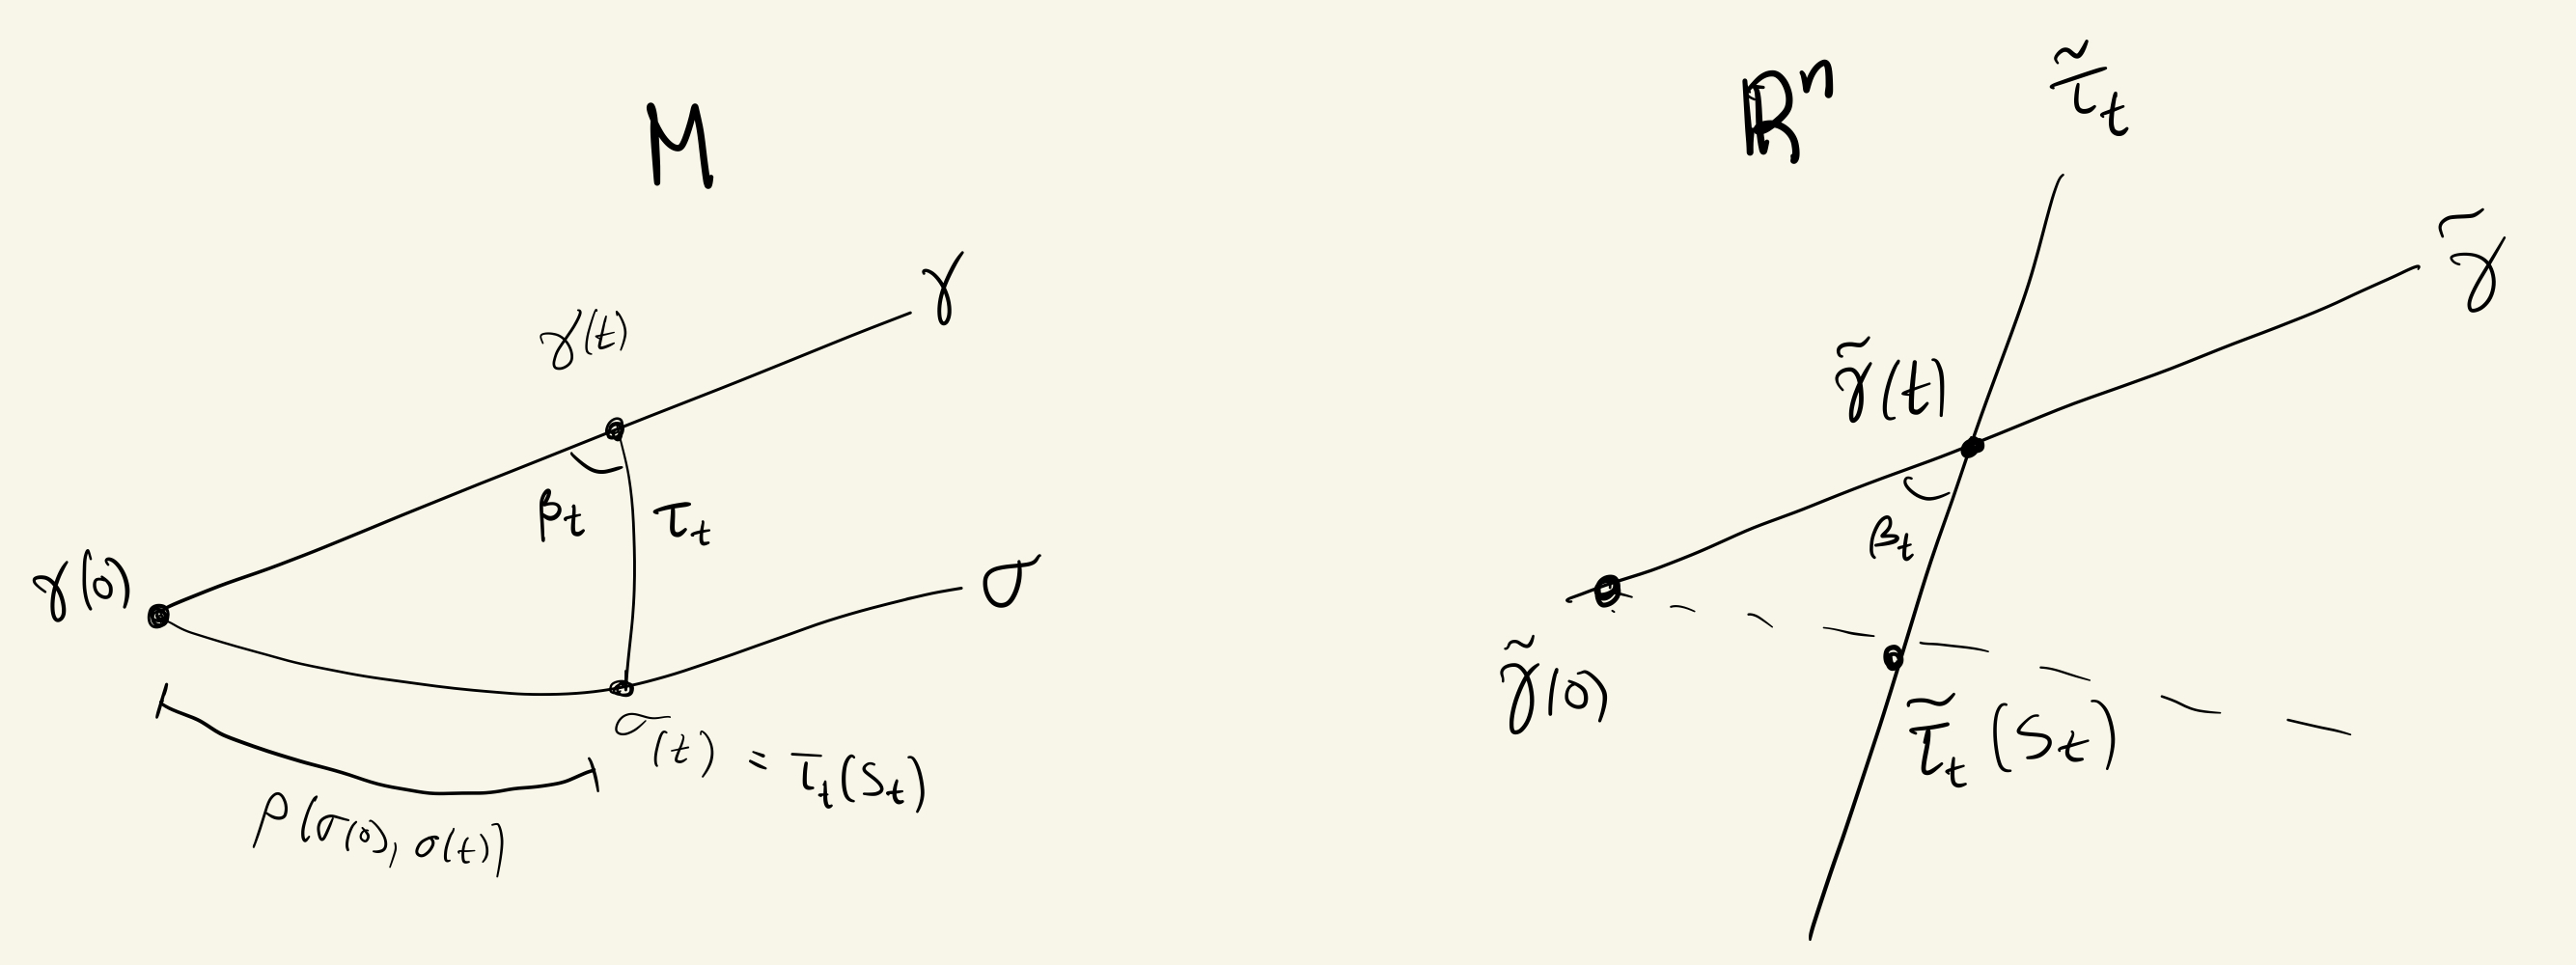
\includegraphics[width=1\textwidth]{figures/toponogov-exercise}
\caption{}
\label{figure-toponogov-exercise}
\end{figure}
Podemos calcular a distância
$\rho_{\mathbb{R}^n}(\tilde{\gamma}(0),\tilde{\tau}_t(s_t))$ usando a lei de
cosenos euclidiana desde que conheçamos $\beta_t$ e $\ell(\tau_t)$:
$$
\rho_{\mathbb{R}^n}(\tilde{\gamma}(0),\tilde{\tau}_t(s_t))^2=
t^2+\ell(\tau_t)^2-2t\ell(\tau_t)\cos \beta_t
$$
Para calcular $\ell(\tau_t)$ podemos usar o Teorema de Toponogov de novo, dessa
vez comparando a hinge $(\gamma'(0), \sigma'(0),\alpha)$ com uma correspondente
no espaço euclidiano:
\begin{figure}[H]
\centering
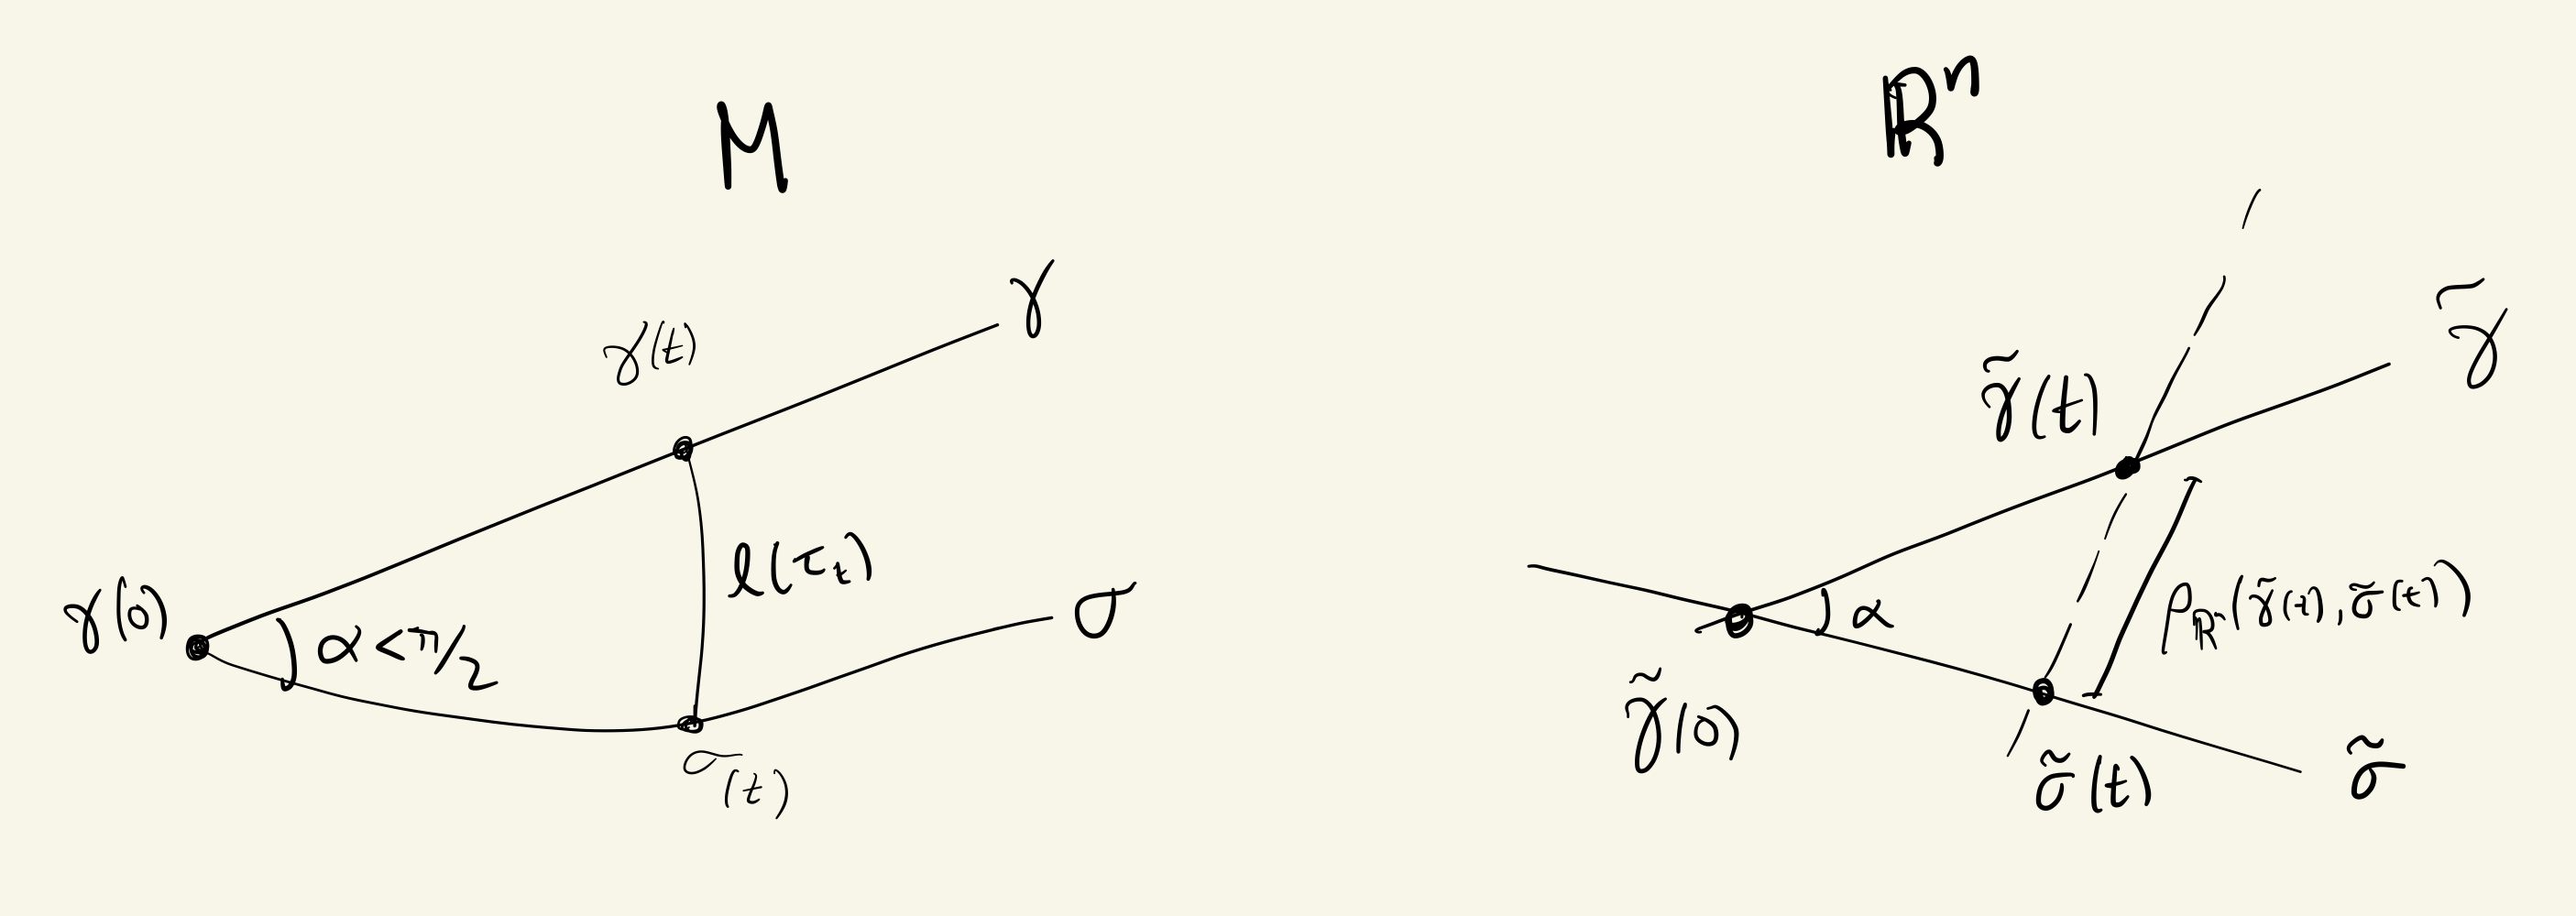
\includegraphics[width=1\textwidth]{figures/toponogov-exercise2}
\label{figure-toponogov-exercise2}
\end{figure}
Obtemos que
$$
\rho_{\mathbb{R}^n}(\tilde{\gamma}(t),\tilde{\sigma}(t))\leq \ell(\tau_t)
$$
Como $\alpha$ é constante conforme $t$ muda, podemos fixar $\tilde{\gamma}$ e
$\tilde{\sigma}$ para fazer a nossa comparação. Conforme  $t$ avança, nos
movemos a velocidade constante ao longo de $\tilde{\gamma}$ en direção ao
infinito, e embora não sabemos se a distância $\rho(\sigma(0),\sigma(t))$ cresse
 ou diminue, a distância do nosso interesse 
$\rho_{\mathbb{R}^n}(\tilde{\gamma}(t),\tilde{\sigma}(t))$
vai sempre crescendo, e concluimos que diverge ao infinito.

Portanto o problema acaba se conseguimos achar uma cota inferior positiva para
$\beta_t$. Parece que isso é equivalente a provar que a distância entre
$\gamma$ e $\sigma$ está acotada inferiormente por uma constante positiva…

A lei de cosenos do lado Euclideano nos diz que
$$
\rho_{\mathbb{R}^n}(\tilde{\gamma}(t),\tilde{\sigma}(t))^2=
t^2+|\tilde{\sigma}(t)|^2-2t |\tilde{\sigma}(t)|\cos \alpha
\leq t^2+|\tilde{\sigma}(t)|^2-2t |\tilde{\sigma}(t)|
$$
Supondo que $\tilde{\gamma}(0)=\tilde{\sigma}(0)=0 \in \mathbb{R}^n$. 
Parece que para medir essa distância deveríamos conhecer
$|\tilde{\sigma}(t)|=\rho(\sigma(0),\sigma(t))$...
 o que parece levar o problema de volta ao
problema inicial.
\end{proof}

\begin{proof}[Prova de \cite{Cheeger-Ebin}]
Por desigualdade triangular, para quaisquer $t,s \in \mathbb{R}$,
$$
\rho(\sigma(t),\sigma(0)) \geq
\rho(\gamma(s),\sigma(t))-\rho(\gamma(s),\gamma(0)).
$$
Como o lado esquerdo não depende de $s$, vemos que basta tomar o limite quando 
$s\to \infty$ e mostrar que esse limite está inferiormente limitado por um
número que depende linearmente de $t$, i.e. $t \cos\alpha$.

Considere uma geodésica minimizante $\tau_{s,t}$ ligando $\gamma(s)$ e
$\sigma(t)$. Podemos usar o teorema de Toponogov \ref{theorem-Toponogov-angle}
na versão de ângulos (que está enunciada em \cite{Cheeger-Ebin}) já que duas das
geodésicas no triângulo $\gamma(0),\gamma(s),\sigma(t)$ são minimizantes por
hipótese. Como a cota inferior da curvatura é 0 não temos problemas com o
comprimento de $\sigma$.

Obtemos que existe um triângulo Euclidiano com lados do mesmo comprimento tal
que os ângulos correspondentes são menores o iguais que os ângulos com que
começamos.

Denote $A:=\rho(\gamma(0),\gamma(s))=s$, $B:=\ell(\sigma(t))=t$ e
 $C:=\rho(\gamma(s),\sigma(t))=\ell(\tau_{s,t})$.
Nosso objetivo é limitar inferiormente $C-A$ conforme  $s \to \infty$.
 Aplicamos a lei de cosenos no lado Euclidiano para obter
\begin{align*}
C^2&=A^2+B^2-2AB\cos\tilde{\alpha}\\
\implies C^2-A^2&=B^2-2AB\cos\tilde{\alpha}\\
\implies C-A&=\frac{B^2-2AB\cos\tilde{\alpha}}{C+A}
\end{align*}
Onde só $A=s$ e $C$ dependem de $s$. O comportamento assintótico desse quociente
quando $s \to \infty$ é claro geometricamente: como $A$ e $C$ são dois lados de
um triângulo, eles crescem proporcionadamente. Formalmente, como $C \leq A+B$,
obtemos $C+A \leq 2A+B$. Daí
\begin{align*}
\frac{1}{C+A}&\geq \frac{1}{2A+B}\\
\implies \frac{B^2-2AB\cos \tilde{\alpha}}{C+A}&\geq
 \frac{B^2-2AB \cos \tilde{\alpha}}{2A+B}
=\frac{A}{A}\frac{B^2/A-2B\cos \tilde{\alpha}}{2+B/A}
\end{align*}
que (a menos de analizar o que acontece se o numerador é negativo…)
 converge a $B\cos \tilde{\alpha}$ conforme $s \to \infty$.
 Concluímos que $C-A$ deve
convergir a $-t\cos\tilde{\alpha}\leq-t\cos\alpha$. Tirando o signo obtemos a
desigualdade desejada.
\end{proof}

\bibliography{my}
\bibliographystyle{amsalpha}

\end{document}

